\section{Piede cavo}

\emph{Per quanto riguarda il piede cavo siamo nella deformità opposta rispetto al piede piatto. Morfologicamente avremo un \textbf{\emph{aumento della volta plantare, una rotazione interna del tallone con una rotazione di tutto l'arto inferiore all'esterno}}, mentre nel piede piatto c'è una rotazione all'interno. Il piede cavo sta tra il piede normale e la massima espressione di eccesso di pronazione, ovvero il piede piatto.}

\subsection{Definizione}

Deformità caratterizzata dal \textbf{punto di vista morfologico} dalla presenza di un \emph{aumento dell'altezza della volta plantare, una rotazione interna del tallone associata a deformità più o meno importante del primo dito e di tutte le dita,} in particolare
\textbf{griffe delle dita} dovute ad uno squilibrio muscolare: il 90\% dei piedi cavi dipende proprio da questo. Da un \textbf{punto di vista funzionale} si intende per piede cavo una \emph{deformità caratterizzata
da una prevalenza o eccesso di supinazione}.

In questa definizione rientrano numerosi quadri clinici con diversi aspetti eziopatologici, anatomopatologici e terapeutici.

\subsection{Eziologia}

Dal punto di vista eziologico si può distinguere il piede cavo in tre forme principali:

\begin{itemize}
\item[1.] Piede Cavo Congenito, fortunatamente di riscontro raro, che si può osservare già dalla nascita e che si manifesta con un marcato equinismo asimmetrico dei metatarsi senza un interessamento del retropiede. Per
quanto riguarda l'origine di questa forma, alcuni autori ipotizzano che la deformità possa essere dovuta a cause genetiche, ma senza un preciso modello di ereditarietà, mentre secondo altri avrebbe un ruolo predominante una qualche alterazione meccanica dovuta a mal posizioni
intrauterine o a squilibri muscolari.

\item[2.] Piede Cavo Secondario (o Acquisito), che è la forma di piede cavo più comune, potendo a sua volta essere distinto in piede cavo neurogeno, miopatico, post-traumatico o degenerativo a seconda della patologia alla
base, e tra queste il più comune è il piede cavo neurogeno, dovuto ad esempio a poliomielite, spina bifida, malattia di Friederich, paralisi spastiche, neuropatie sensitivo-motorie e malattia di Charcot-Maria-Tooth.

\item[3.] Piede Cavo Essenziale (o Idiopatico), in cui non è possibile identificare una causa specifica alla base. Un tempo queste forme rappresentavano l'80\% delle forme di piede cavo, mentre oggi, grazie alla moderne tecniche diagnostiche, la percentuale è scesa al solo 10\%.
\end{itemize}

\begin{itemize}
\item
  \emph{\textbf{Malattie neurologiche}} (man mano che la neurologia si è evoluta in termini di diagnosi le percentuali di piede cavo idiopatico si sono notevolmente ridotte). Malattie come l'atassia spinocerebellare, la malattia di Charcot Marie Tooth, la poliomielite, la paralisi spastica infantile possono comunque dare una deformità in cavismo sempre mediata da uno squilibrio muscolare dei muscoli della gamba sull'azione sul piede.
\item
  \emph{\textbf{Malattie muscolari}} (miopatie, distrofia muscolare di Duchenne)
\item
  \emph{\textbf{Malattie vascolari}}: ad esempio \textbf{retrazione ischemica di Volkmann} che c'è nella mano e anche nel piede. Si ha una sproporzione tra il tempo di ischemia e quella di vascolarizzazione che crea la possibilità che i muscoli vadano in necrosi e che ci sia quindi una retrazione di alcuni muscoli e questo crea il piede cavo.
\item
  \emph{\textbf{Fratture }}
\item
  \emph{\textbf{Malattie reumatiche:}} l'artrite reumatoide dà delle deformità più o meno tipiche prevalentemente legate al piede piatto perché crolla tutto, il ginocchio e il piede vanno in valgo. Ci sono però alcune forme di reumatismi infiammatori cronici che non sono artrite reumatoide, dove la componente di disallineamento è minore, come la sindrome di Reiter, reumatismo psoriasico. In queste forme la tendenza non è quella a crollare, ma ad avere delle retrazioni e delle ``mummificazioni''. Alle volte può svilupparsi in associazione ad artrite reumatoide in quanto nulla vieta che uno abbia un piede cavo da prima e che a 30 anni sviluppi artrite reumatoide.
\end{itemize}

\begin{figure}[!ht]
\centering
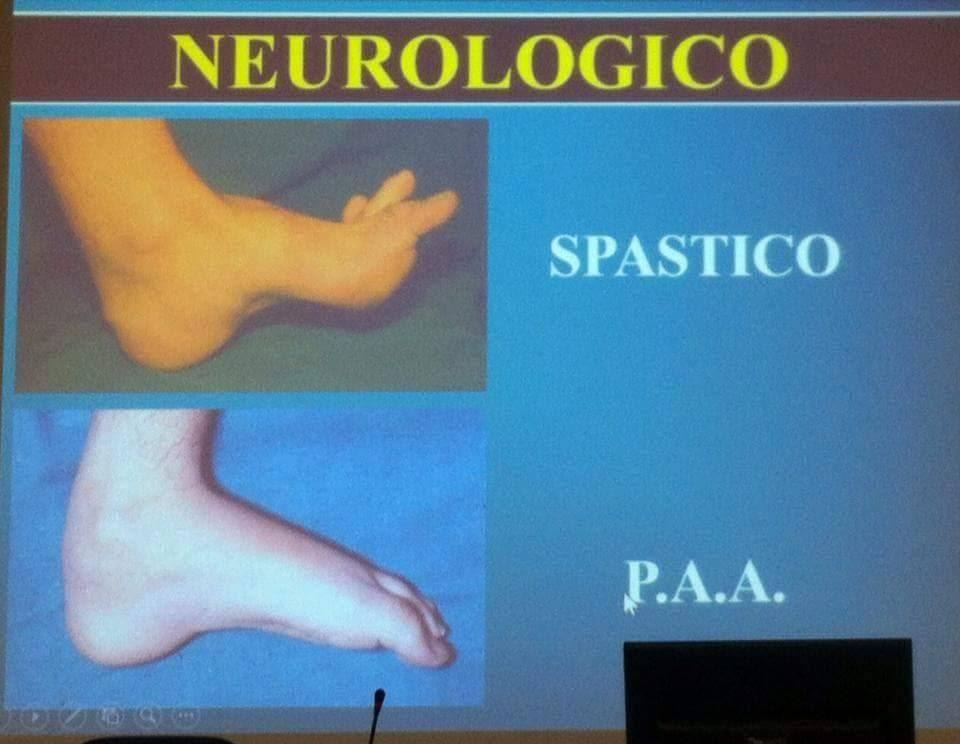
\includegraphics[width=0.4\textwidth]{017/image1.jpg}
\end{figure}

Nel piede cavo da poliomielite c'è una assoluta mancanza del tricipite e il calcagno, non essendo più sostenuto dal tono muscolare del tricipite, va giù determinando un cavismo oltre ad una paralisi dei muscoli anteriori della gamba.

Qui si può osservare l'esito di una fasciotomia. Se la frattura è data da un trauma che ha solo leso l'osso, può non succedere niente, ma se si tratta di un trauma importante per cui c'è stata una trazione dei muscoli e un notevole aumento di volume, si crea la cosiddetta \textbf{sindrome compartimentale}. I muscoli sono contenuti in compartimenti inestensibili quindi se questi gonfiano dentro queste fasce, la pressione compartimentale aumenta e le arterie si chiudono con conseguente gangrena. Per ridurre la pressione compartimentale può essere messa in atto una fasciotomia. Quando questo non avviene i muscoli vanno in sofferenza, c'è una trazione di alcuni muscoli rispetto ad altri e ciò crea uno squilibrio muscolare che porta al piede cavo.

\begin{figure}[!ht]
\centering
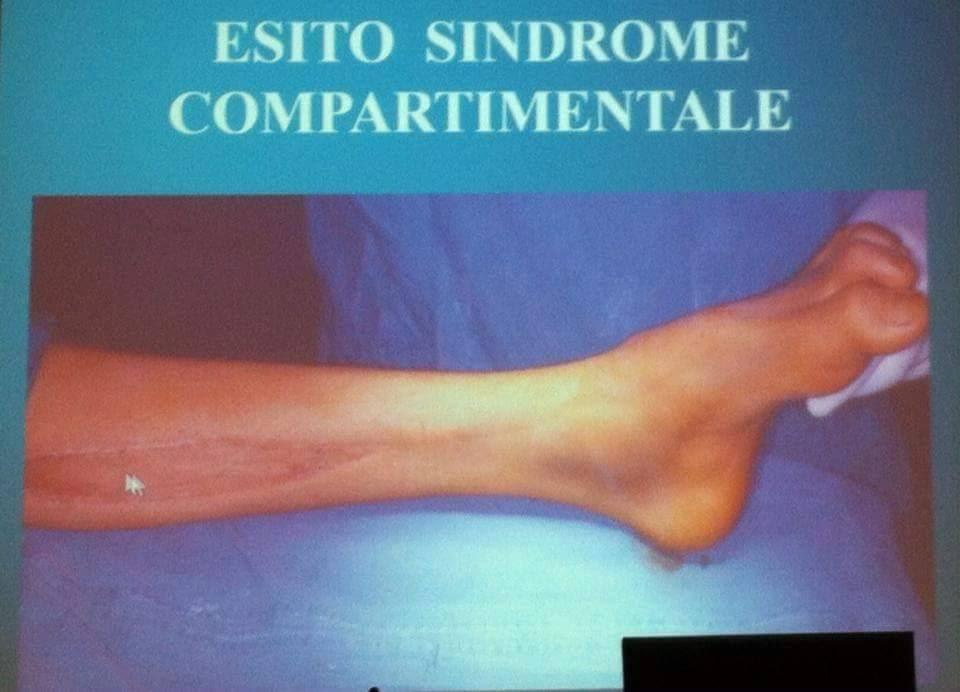
\includegraphics[width=0.4\textwidth]{017/image2.jpg}
\end{figure}

\begin{figure}[!ht]
\centering
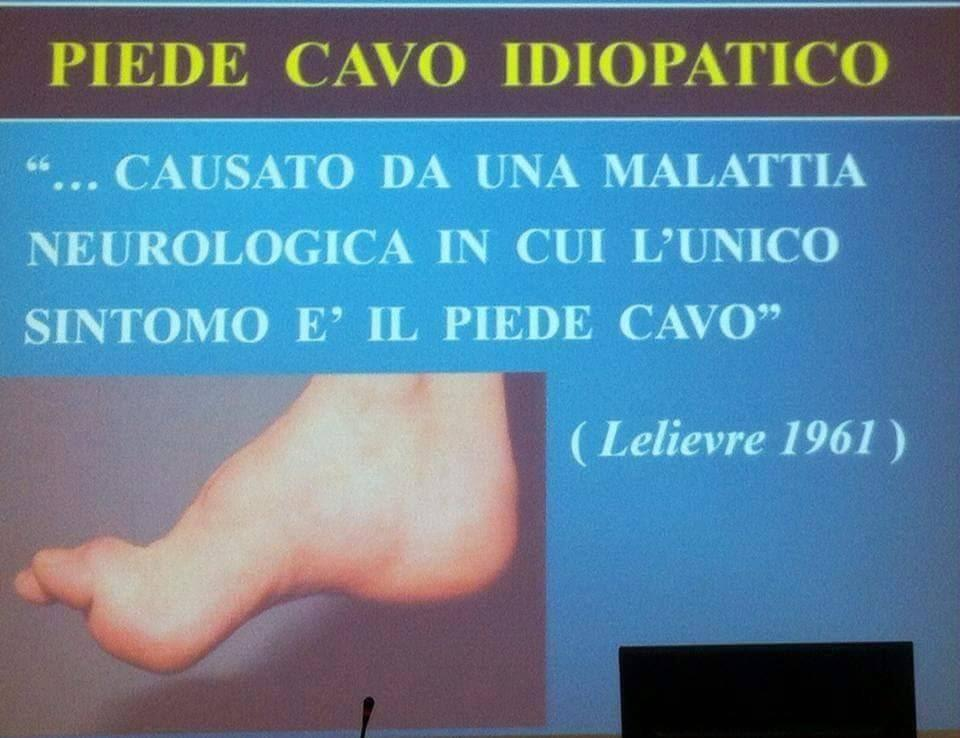
\includegraphics[width=0.4\textwidth]{017/image3.jpg}
\end{figure}

\begin{figure}[!ht]
\centering
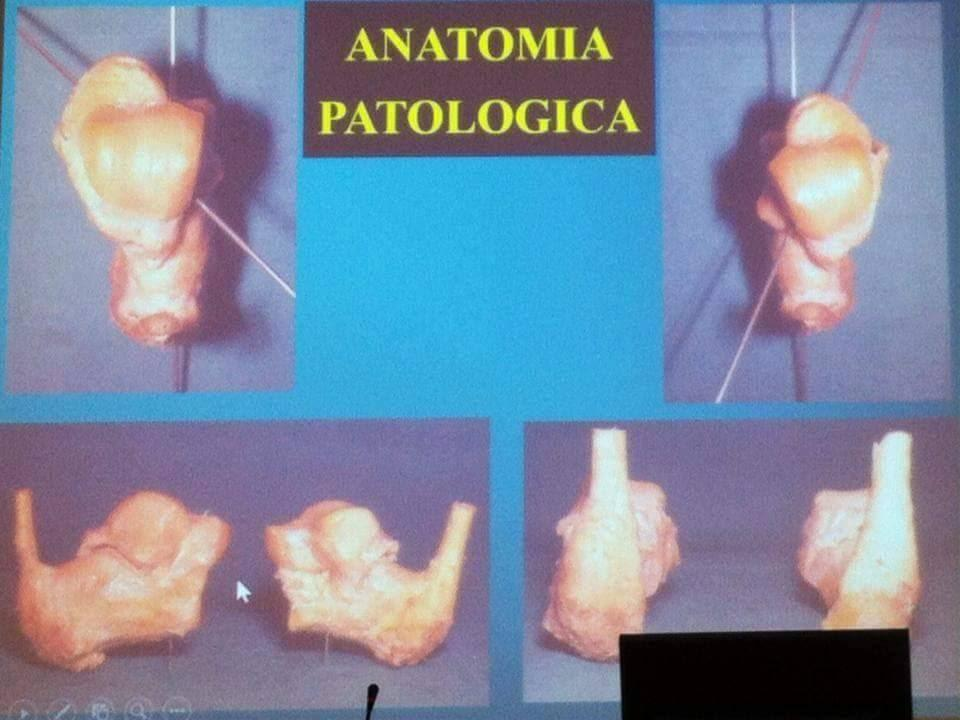
\includegraphics[width=0.4\textwidth]{017/image4.jpg}
\end{figure}

\emph{(Dalla foto si può notare che mentre nel piede piatto c'è un astragalo che ruota all'interno e va giù perché il calcagno va all'esterno, nel piede cavo è il contrario, l'astragalo è più su ed extra ruotato insieme a tutto l'arto inferiore, rispetto al piede.)}

(foto)

\subsection{Patogenesi}

Osservando lo schema a destra, vediamo che le barrette sono le ossa, i pallini le articolazioni mobili, le frecce i muscoli da immaginare come degli elastici. Una articolazione possiamo accomunarla alla metatarso falangea dell'alluce, una alla mediotarsica e l'altra all'articolazione della caviglia. Il piede riesce a mantenere la sua forma, quella normale, perché tutti i muscoli si ritrovano in equilibrio. Nel piede cavo ci possono essere diverse progressioni come ad esempio, \emph{un tibiale anteriore che funziona meno non trattiene il primo metatarsale che va in basso dando una forma di piede cavo antero-interno} perché gli altri metatarsi, diversamente dal primo, non sono andati giù. Abbiamo quindi uno squilibrio di tutte le altre articolazioni con comparsa della \textbf{griffe del primo dito}. Poi c'è una \emph{progressione disto-prossimale}. Ci sono alcune patologie che colpiscono i muscoli lombricali e interossei del piede con squilibrio disto-prossimale.
Esiste anche una possibilità di progressione combinata prossimale e distale della deformità.

\begin{figure}[!ht]
\centering
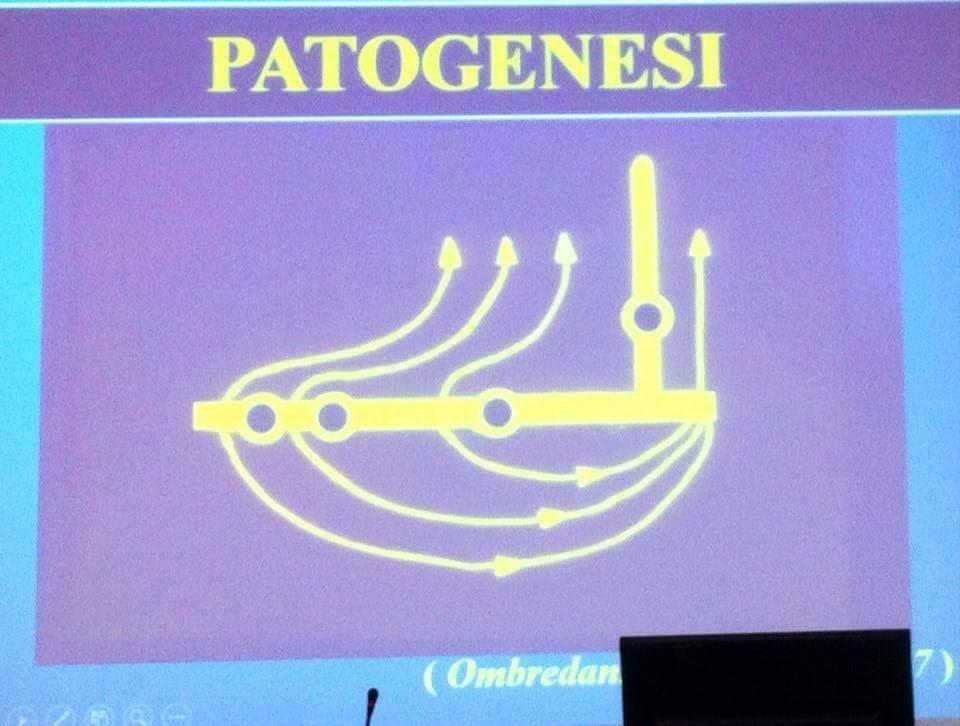
\includegraphics[width=0.4\textwidth]{017/image5.jpg}
\end{figure}

\subsection{Evoluzione di un piede cavo idiopatico }

\begin{figure}[!ht]
\centering
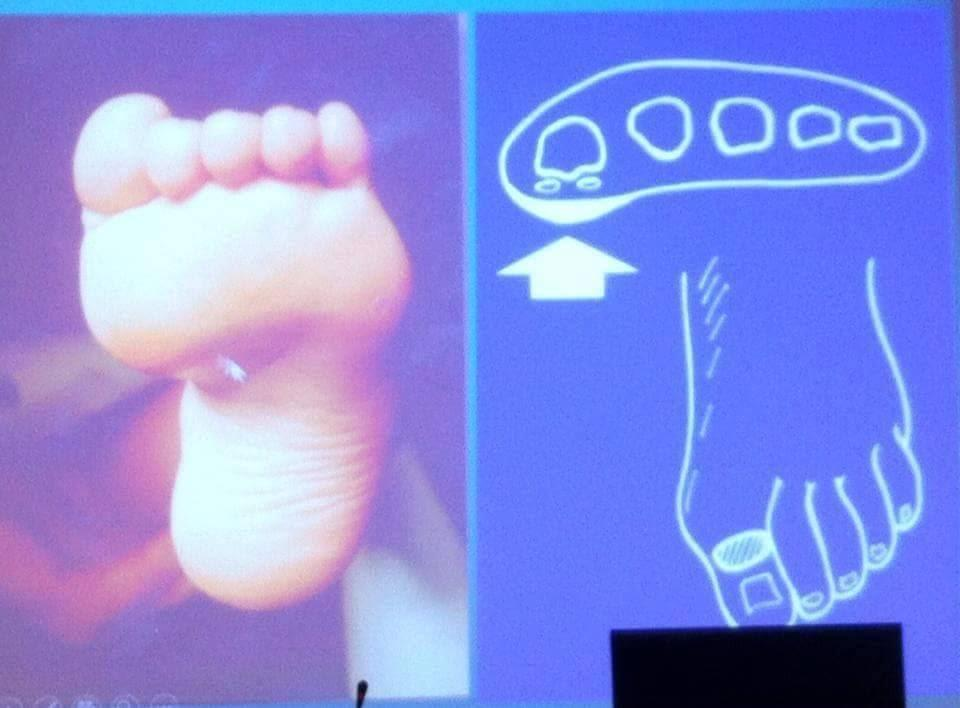
\includegraphics[width=0.4\textwidth]{017/image6.jpg}
\end{figure}

\begin{figure}[!ht]
\centering
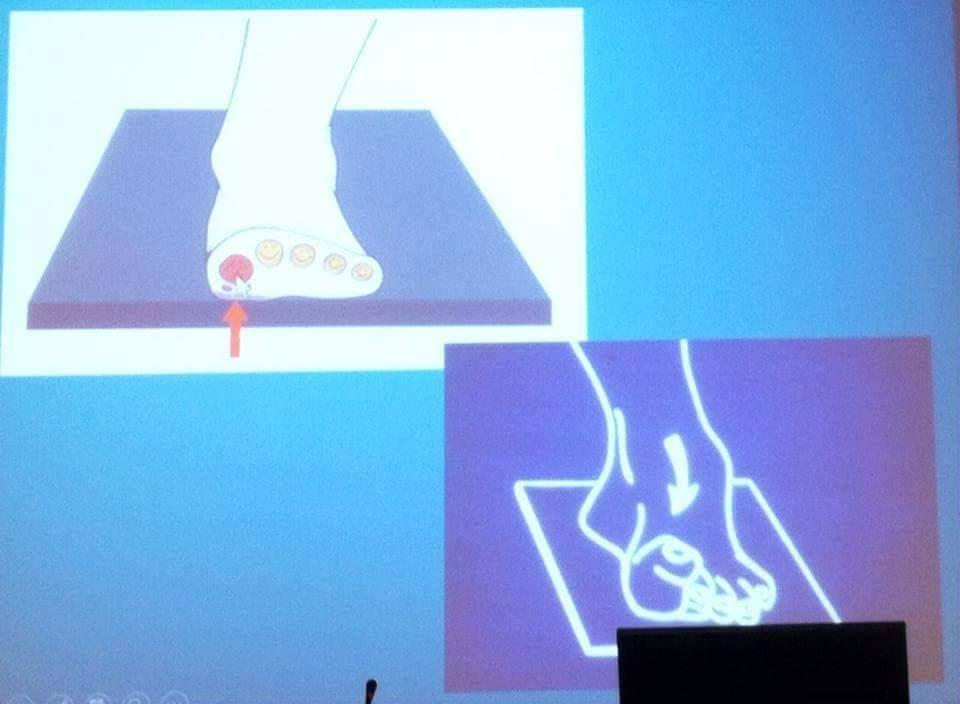
\includegraphics[width=0.4\textwidth]{017/image7.jpg}
\end{figure}

\begin{figure}[!ht]
\centering
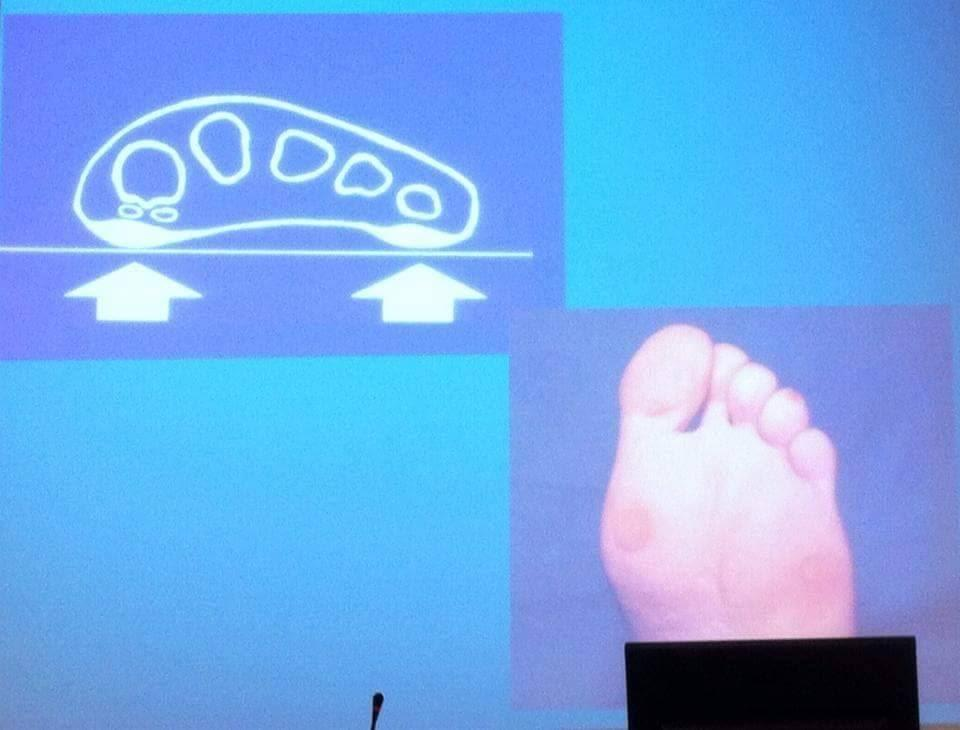
\includegraphics[width=0.4\textwidth]{017/image8.jpg}
\end{figure}

\begin{figure}[!ht]
\centering
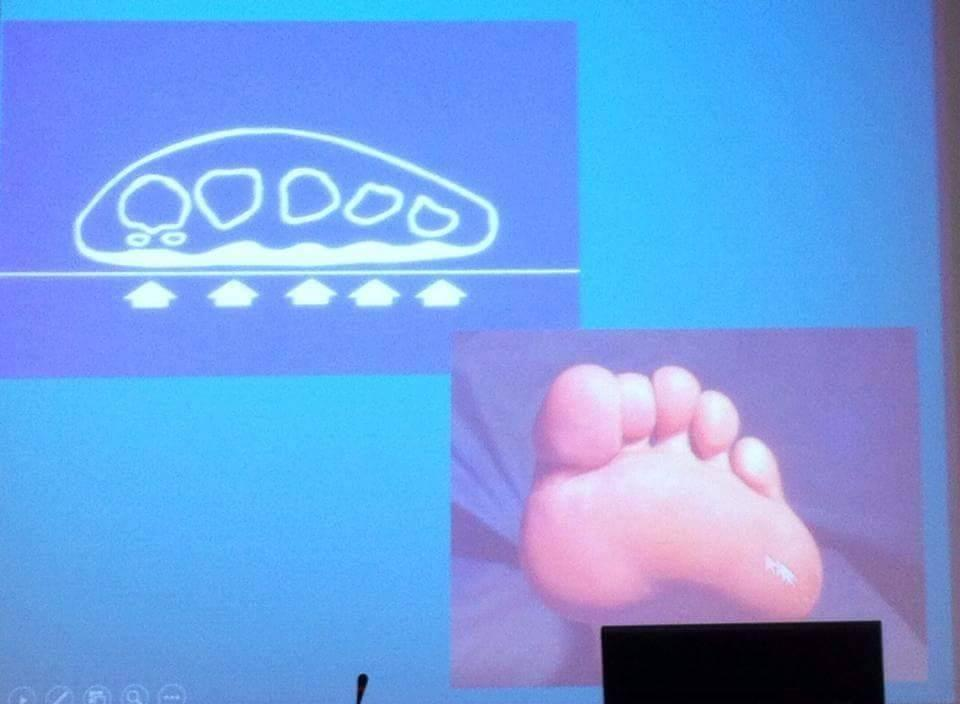
\includegraphics[width=0.4\textwidth]{017/image9.jpg}
\end{figure}

\subsubsection{Clinica}

Il quadro clinico nel bambino e nell'adulto è differente. \textbf{Nel bambino} siccome le articolazioni sono mobili, \emph{in scarico si vede un aumento della volta plantare che scompare sotto carico}. Con il passare del tempo le articolazioni diventano rigide e la deformità si struttura. Il piede si presenta tozzo, comincia a comparire un \textbf{callo} sotto la testa del primo metatarsale, la \textbf{griffe del primo dito} e una \textbf{callosità dorsale da sfregamento della calzatura della prima metatarso falangea}. Questa rigidità del primo
metatarsale determina quello che è \emph{l'effetto tripode}. Uno dei segni del piede cavo è infatti l'\emph{instabilità}. I pazienti infatti, vanno facilmente incontro a distorsione del retropiede perché hanno un
assetto con appoggio prevalentemente esterno e quindi difficilmente riescono a far fronte ad una supinazione addizionale come, ad esempio, quando si corre o si mette il piede in una buca. A forza di avere questo effetto tripode, compare una callosità sul quinto metatarsale con
comparsa di un arco metatarsale trasverso che normalmente non è presente, in quanto i metatarsali devono avere tutti uno stesso appoggio. \emph{Successivamente} si ha la caduta di tutti i metatarsali con \textbf{callosità su tutto il tallone anteriore}. La caduta di tutto
l'avampiede crea uno squilibrio a livello dei muscoli interossei, lombricali ed estensori con comparsa di una estensione forzata della falange basale e una flessione forzata delle falangi distali con formazione della griffe. Compare anche metatarsalgia che viene ulteriormente peggiorata dalla griffe delle dita. Se si verifica
un'evoluzione segue questo decorso, ma non è detto che ciò avvenga.

Clinicamente si possono distinguere:
\begin{itemize}
\item Piede Cavo Anteriore, che si caratterizza per una deformità dell'avampiede, mentre il retropiede mantiene la posizione normale, così che si viene a formare un eccessivo slivellamento in basso dell'avampiede rispetto al retropiede che supera il valore fisiologico di 1 cm. Questa forma può essere simmetrica (tutti i metatarsi si
equinizzano allo stesso modo) o asimmetrica (l'equinismo ha un'entità differente per ciascun metatarso).
\item Piede Cavo Posteriore, come si osserva nelle forme paralitiche che interessano il tricipite surale. Questa paralisi determina infatti una talizzazione del calcagno, che nelle forme più marcate giunge anche a vertalizzarsi.
\item Piede Cavo Misto, caratterizzato da cavismo associato anteriore e posteriore.
\item Piede Cavo Antero-Interno, che si caratterizza invece per la caduta in equinismo del 1\textsuperscript{o} metatarsale, mentre gli altri rimangono in posizione,
con conseguente pronazione dell'avampiede e dal varismo del retro piede.
\end{itemize}

\subsubsection{Sintomatologia}

\begin{itemize}
\item
  Anomalie della marcia
\item
  Frequenti cadute
\item
  Alterazioni del rapporto con la calzatura
\item
  Deformità
\item
  Dolore
\end{itemize}

Nel \emph{piede cavo idiopatico} abbiamo una prevalente caduta dell'avampiede rispetto al retropiede, in quello della poliomielite una caduta del retropiede.

\begin{figure}[!ht]
\centering
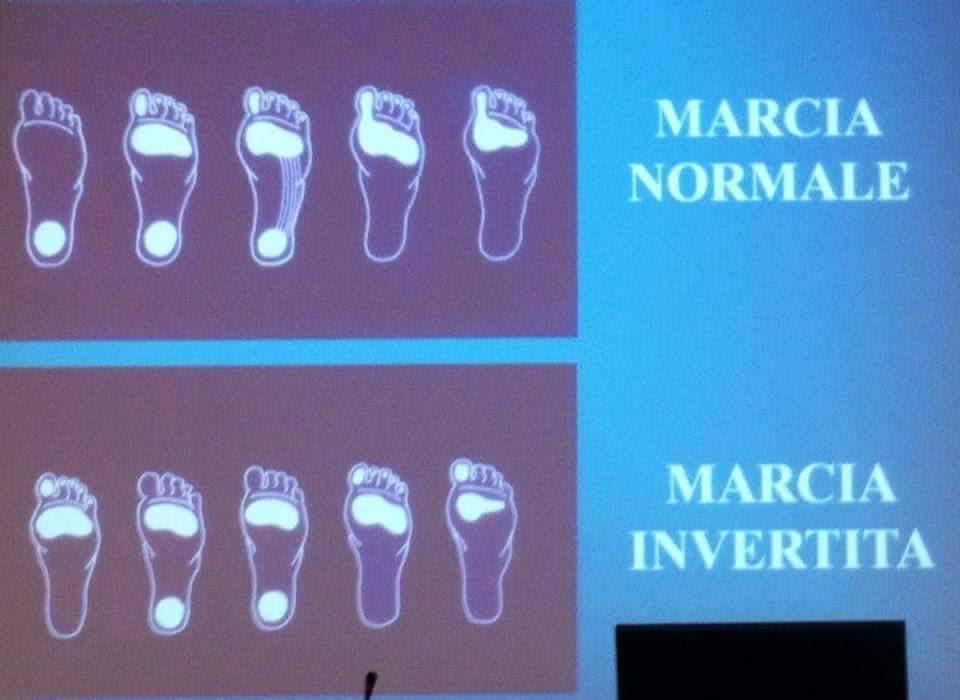
\includegraphics[width=0.4\textwidth]{017/image10.jpg}
\end{figure}

Il paziente presenta un'alterazione della marcia normale (arrivo con il tallone - appoggio il tallone anteriore - trasferimento di carico dal retropiede all'avampiede - spinta dell'avampiede fino all'alluce ). Nel piede cavo c'è una \textbf{\emph{marcia invertita}} a causa della caduta dell'avampiede rispetto al retro piede. Prima tocca l'avampiede, poi il retropiede e poi una fase di spinta anche diminuita, se la deformità è grave. Il piede cavo è un piede ``pronto'', infatti è molto comune negli atleti. Se c'è un piede cavo neurologico, l'alterazione dinamica è
primitiva e l'alterazione morfologica è secondaria; mentre, se è dovuto ad una frattura con causa osteo-articolare, primitiva è l'alterazione morfologica e secondaria quella dinamica.

\begin{figure}[!ht]
\centering
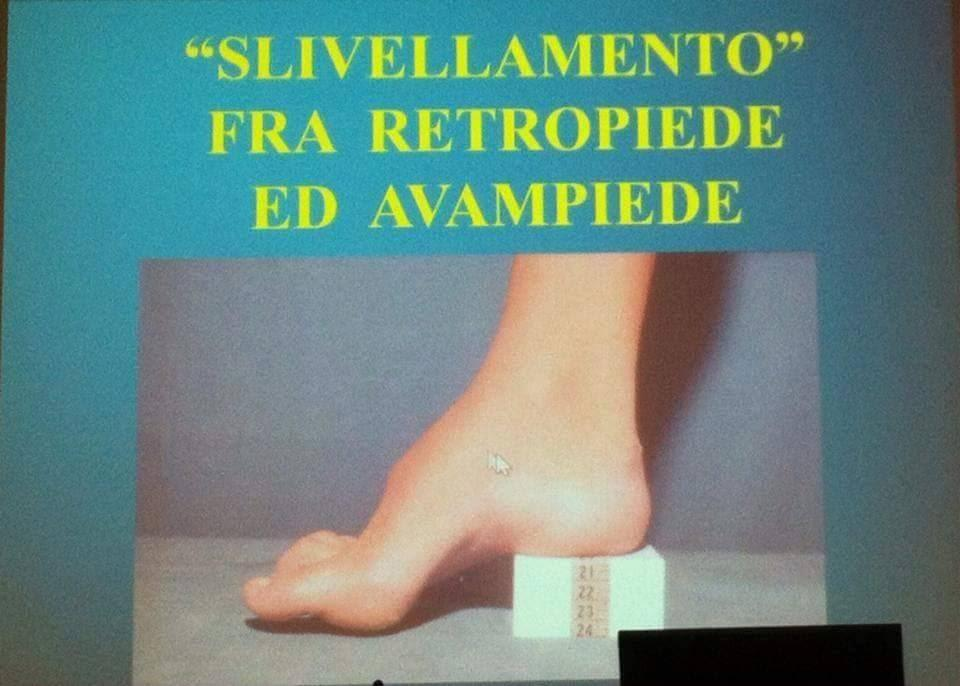
\includegraphics[width=0.4\textwidth]{017/image11.jpg}
\end{figure}

Utilizzando un rialzino di alcuni centimetri sotto il tallone, si può riportare la caviglia in posizione normale ovvero ad angolo retto e con il tallone orizzontale. Essendoci un cavismo prevalentemente anteriore \textbf{l'avampiede è slivellato rispetto al retro piede} quindi, per avere una posizione neutra della caviglia ho bisogno di un tacco.
Togliendo il rialzo, abbiamo una deformità rigida e per poter poggiare il tallone, \emph{la caviglia va in flessione dorsale con conseguente
dolorabilità nella parte anteriore della caviglia}. Questo perché
l'astragalo davanti è più largo rispetto alla coda quindi ogni volta che il piede va in flessione dorsale la pinza tibio-peroneale si apre, costringendo la parte anteriore dell'astragalo continuamente all'interno della pinza e costringendo, inoltre, a trazione continua i legamenti
della caviglia. Quindi senza tacco tutto il sistema calcaneo - achilleo - plantare è in trazione continua con conseguente fastidio. Infatti, si hanno tendinopatie d'Achille, fascite plantare.

\subsubsection{Diagnosi}

\begin{itemize}
\item
  Esame generale
\item
  Esame della marcia
\item
  Esame del piede
\item
  Esame della calzatura
\end{itemize}

Non bisogna mai fermarsi alla semplice osservazione. Fare diagnosi vuol dire \emph{\emph{tipizzare il piede in funzione del paziente}}. Bisogna analizzare tutte le variabili, scovare se esiste una malattia di fondo
(il più delle volte sono neurologiche). E' importante fare un buon \textbf{esame neurologico}, questo serve per vedere innanzitutto il tipo di malattia ma, soprattutto, per sapere la possibile evoluzione.
Infatti, se il paziente presenta una malattia stabilizzata dal punto di vista dello squilibrio muscolare, si può pensare ad un intervento, cosa che risulta inutile in un paziente in cui la malattia non si è ancora manifestata completamente. In pazienti con piede cavo bisogna sempre
chiedere una \textbf{radiografia del rachide lombo-sacrale}, infatti il più delle volte si ritrova una schisi vertebrale oppure una qualche \emph{malformazione del passaggio lombo-sacrale} (clinicamente si può
osservare un ciuffo di peli a livello lombare basso).

\paragraph{Valutazione ortopedica (esame del piede)}:

\begin{itemize}
\item
  \emph{Riducibilità del varismo del tallone}: mentre il piede piatto ha un tallone ruotato all' esterno, nel cavo è ruotato all' interno spesso a causa di ~una caduta del primo metatarsale per l' effetto tripode. Devo capire quindi, se questa rotazione del calcagno è dovuta a questo oppure è una componente della deformità.
\item
  \emph{Riducibilità della deformità}
\item
  \emph{Valutazione motilità articolare e lo stato delle articolazioni}: se le articolazioni sono rigide e artrosiche non conviene salvarle in quanto, il più delle volte, dolenti; al contrario, se esiste ancora una mobilità, bisognerà pensare ad interventi che interessino o le parti molli o che non tocchino le articolazioni evitando di ridurre quella che è la mobilità del piede.
\item
  \emph{Riducibilità della deformità delle dita}
\end{itemize}

\paragraph{Giusto modo di visitare un piede}
Si mette la tibio-tarsica in posizione neutra, si corregge il varismo del retropiede con cui viene fuori tutta la caduta del primo metatarsale. Quando i pazienti tirano su il piede la griffe del primo dito peggiora cosa che non avviene in un piede normale. Si possono apprezzare le varie callosità e anche l' evidenza dei tendini sottocutanei.

\emph{Come faccio a capire se il calcagno è varo perché è caduto il primo metatarsale o perché c'è una deformità alla base?}

Esiste il test di \textbf{COLEMAN-ANDREASI} che mi permette di orientare la terapia. Se il paziente presenta un varismo strutturato che dipende dal calcagno, sarà necessario raddrizzare il calcagno. Se dipende dal primo metatarsale invece, si dovrà agire su quest'ultimo. \emph{Per effettuare questo test si prende un gradino, il paziente posiziona l'avampiede nel vuoto escludendolo dal carico e poggia il retropiede sul gradino.
In questa posizione il varismo si riduce qualora dipenda dal primo metatarsale con effetto tripode.}

\paragraph{ESAME RADIOGRAFICO (principali proiezioni)}:

\begin{itemize}
\item
  TIBIO-TARSICA antero-posteriore
\item
  PIEDE DORSO-PLANTARE
\item
  PIEDE LATERALE
\end{itemize}

\paragraph{Radiografia tipica}
Notiamo \emph{astragalo orizzontale, calcagno impennato, dorso del piede aumentato, griffe delle dita}.
L'astragalo è ruotato verso l'esterno, il calcagno verso l'interno. Con la proiezione dorso-plantare si può osservare il cavismo associato a adduzione dell'avampiede e affastellamento dei metatarsali. In proiezione laterale pura si osserva il perone molto indietro rispetto alla tibia. Lo squilibrio tra avampiede e retropiede con conseguente flessione dorsale della tibio-tarsica, a lungo andare determina un impingement (reazione osteofitosica). La rotazione esterna dell'astragalo si porta dietro tutta la gamba e quindi porta anche ad una rotazione esterna del ginocchio (strabismo divergente delle rotule) e dell'anca.

Sulla radiografia possono essere fatte anche delle misurazione che comunque lasciano il tempo che trovano. Si può osservare che, anziché avere i normali 120 gradi tra asse della tibia e asse dell'astragalo, si arriva quasi a 90.

Per quanto riguarda la diagnostica per immagini, è molto importante a fini diagnostici un Rx che consenta di valutare l'entità dell'angolo di Costa-Bertani, che viene calcolato in proiezione latero-laterale tracciando prima una linea che parte dal punto più basso della tuberosità posteriore del calcagno ed arriva al punto più basso della testa dell'astragalo, mentre una seconda linea va dalla testa dell'astragalo sino al punto più basso del sesamoide interno dell'alluce; in condizioni normali l'angolo formato da queste due linee si aggira tra i 125\textsuperscript{o} ed i 130\textsuperscript{o}, mentre nel piede cavo l'angolo è notevolmente ridotto.

TAC e RMN sono poco utili a meno che non si vogliano valutare delle fusioni o mancate segmentazioni.

\paragraph{Esami complementari}

\begin{figure}[!ht]
\centering
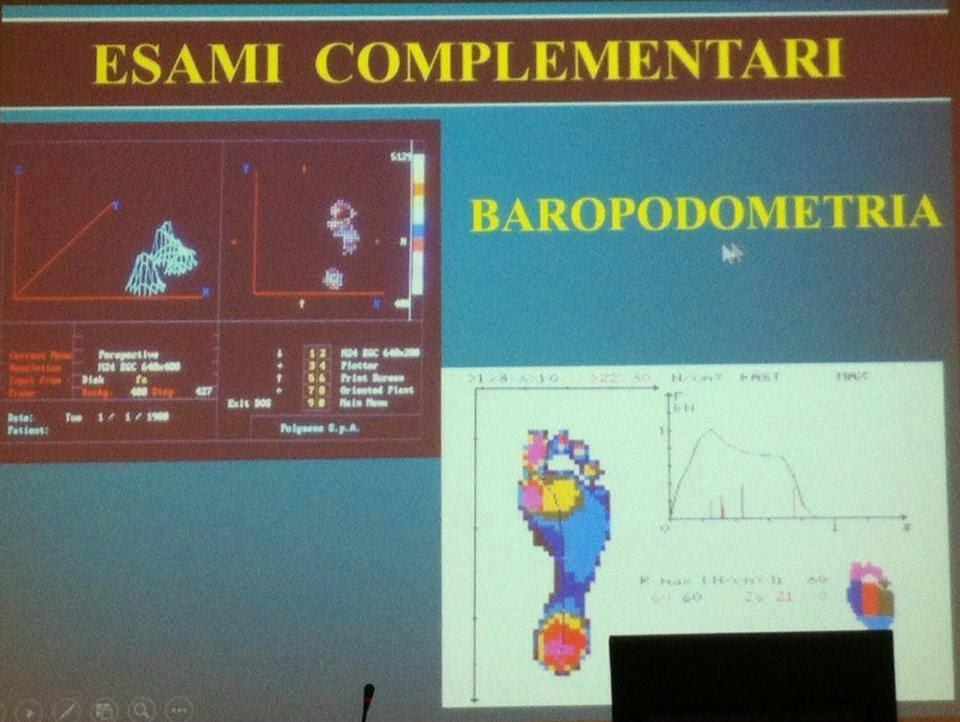
\includegraphics[width=0.4\textwidth]{017/image12.jpg}
\end{figure}

\begin{figure}[!ht]
\centering
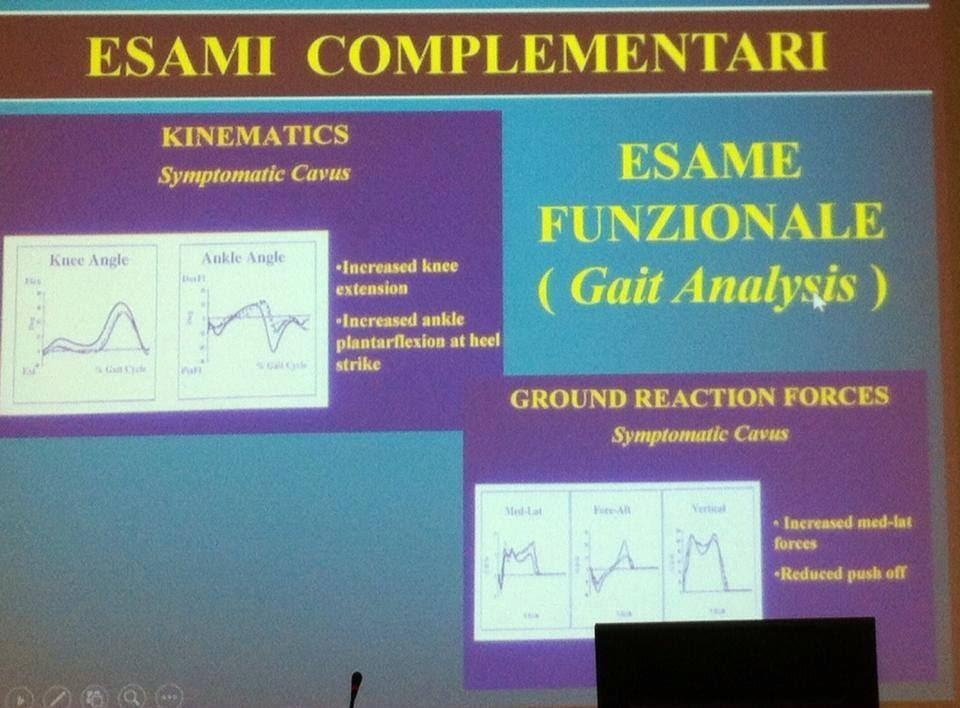
\includegraphics[width=0.4\textwidth]{017/image13.jpg}
\end{figure}

\subsubsection{Trattamento}

\begin{itemize}
\item
  RIABILITATIVO
\item
  ORTESICO~
\item
  CHIRURGICO
\end{itemize}

\textbf{Nel bambino}: nella maggior parte dei casi non ho ancora una rigidità, esiste quindi una certa riducibilità.
\begin{itemize}
\item \textbf{Trattamento riabilitativo}:
\begin{itemize}
\item
  stretching delle parti molli (allungamento dell' aponeurosi plantare per far si che la sua retrazione non aumenti la volta plantare)
\item
  rieducazione alla marcia
\end{itemize}
\item \textbf{Trattamento ortesico}:
\begin{itemize}
\item
  compensare il piede
\item
  riequilibrare il carico sotto le teste metatarsali con una barra
\item
  favorire la fase di spinta che viene persa con la griffe delle dita
\item
  ridurre il dolore
\end{itemize}

C'è la possibilità di un plantare che non ha la stessa funzione svolta nel piede piatto dove si spera in una correzione. Nel piede cavo non ho la correzione della deformità. Utile anche l' utilizzo di un rialzo al tacco per riequilibrare la situazione.

\item \textbf{Trattamento chirurgico}:

Nel bambino sono interventi che non toccano le articolazioni e che interessano il meno possibile l' osso per evitare disparità durante l'accrescimento.

\begin{itemize}
\item
  release delle parti molli
\item
  trasposizioni tendinee
\item
  tecniche sull' osso
\item
  tecniche combinate
\end{itemize}
\end{itemize}

L\emph{e tecniche chirurgiche ci interessano poco}: si può effettuare una \textbf{\emph{fasciotomia plantare}} con possibilità di tagliare l'aponeurosi plantare che può essere fatta anche per via percutanea (è un intervento molto pericoloso perchè qui vicino passa l' arteria plantare mediale), \textbf{\emph{allungamento del tendine d' Achille}} come nel piede piatto; se c'è una deformità riducibile delle dita si può intervenire con la \textbf{\emph{sezione dei flessori delle dita o degli estensori}}; se c'è una caduta prevalente del primo metatarsale si può fare una \textbf{\emph{osteotomia del primo metatarsale}} in modo da sollevarlo; se c'è una griffe del primo dito, l'estensore dell'alluce agisce in favore di deformità quindi bisogna portarlo ad agire in favore di correzione. Viene quindi tagliato, suturato al pedidio e l' estensore viene trapiantato a livello del collo del primo metatarsale in modo da tirarlo su; se c'è una deformità strutturata del retropiede bisogna fare una \textbf{\emph{osteotomia valgizzante}}, si prende la tuberosità posteriore e si sposta lateralmente in modo da riequilibrare il carico posteriore.

\textbf{Nell'adulto}:
\begin{itemize}
\item trattamento ortesico:
\begin{itemize}
\item
  ridurre il dolore
\item
  compensare il piede (plantari)
\item
  stabilizzare il piede
\item
  ridurre l' effetto tripode
\end{itemize}
\item trattamento chirurgico:
\begin{itemize}
\item
  correggere la deformità
\item
  limitare il dolore
\item
  mantenere la motilità
\item
  migliorare l' utilizzo del movimento della caviglia che è sempre in posizione di fine corsa.
\end{itemize}
\item FATTORI DI TIPIZZAZIONE:
\begin{itemize}
\item
  eziologia
\item
  età~
\item
  sesso~
\item
  grado di cavismo
\item
  apice della deformità
\item
  motilità
\item
  presenza di artrosi
\end{itemize}
\end{itemize}
